\section{Mecánica}

\subsection*{Engranajes}

Si están en un mismo eje, la frecuencia angular $\omega$ es constante. Si están en contacto o enlazados por una cadena, las velocidades tangenciales $v_t$ son iguales.


\subsection*{Biela-manivela}

Plantear los movimientos circulares. Lo principal es que el riel puede pensarse como el movimiento circular con respecto a otro punto, que se obtiene al extender la manivela y una recta perpendicular al riel.


\subsection*{Grados de libertad}

La fórmula de Grübler da la relación entre los grados de libertad ($F$), el número de barras/eslabones ($n$), las cuplas completas ($j$), las semicuplas ($j'$) y las barras/eslabones anclados al suelo ($G$).

$$F = 3n - 2j - j' - 3G$$

En $j$ y $j'$ se pone el orden de la junta (barras/eslabones incidentes - 1).

\begin{figure}[H]
    \centering
    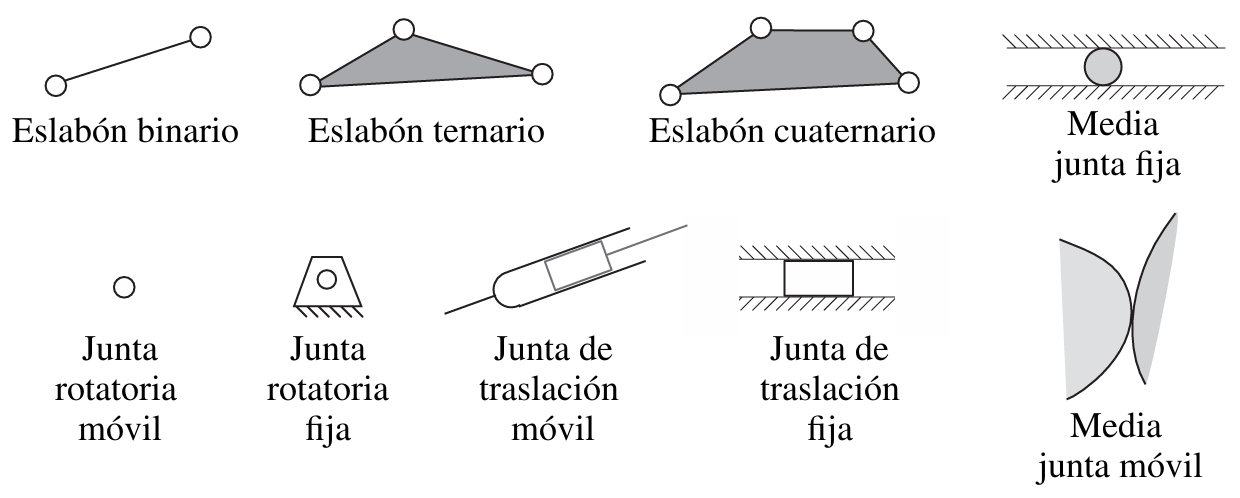
\includegraphics[width=0.7\linewidth]{Images/juntas.png}
\end{figure}

\subsubsection*{Teorema de Grashoff}

En una cadena cinemática de 4 barras, teniendo una fija al suelo, el teorema dice la condición suficiente para que al menos una barra pueda girar completamente (haya al menos una manivela):
$$
S + L \leq P + Q
$$

Donde $S$ y $L$ son el largo de la barra más corta y más larga; y $P$ y $Q$ son las del medio. El bastidor/bancada es la barra fija, una manivela es una barra que puede dar revoluciones completas, un balancín es una barra que no puede completar la vuelta, y el acoplador/biela es la barra que no está unida al bastidor.

Un recurso muy bueno para visualizar cadenas cinemáticas de 4 barras: {\color{blue}\url{https://singsurf.org/things/fourbar.php}}
